	\markboth{CAPITOLO 1. ESERCIZI A.A. 2017-18}{CAPITOLO 1. ESERCIZI A.A. 2017-18}
	\begin{flushleft}
		\textbf{Esercizio 1.1} \textit{Sia }$x = e \approx 2.7183 = \tilde{x}.$ \textit{Si calcoli il corrispondente errore relativo }$\varepsilon_x$ \textit{e il numero di cifre significative k con cui} $\tilde{x}$ \textit{approssima x. Si verifichi che}\\
		\begin{center}
				$ |\varepsilon_x| \approx \displaystyle \frac{1}{2}10^{-k}. $ \\
		\end{center}
		\medskip{}
		\textbf{Soluzione:} Ricordiamo la definizione di \textit{errore relativo}
			\begin{center}
				 $ \varepsilon_x = \displaystyle \frac{\tilde{x} - x}{x} $
			\end{center}
			Il numero di Nepero \textit{e} in MatLab rappresentato tramite la funzione \textit{exp(1)} �:
			\begin{center}
			2.718281828459046
		\end{center}
		Applicando la definizione abbiamo:
		\begin{center}
			$|\varepsilon_x| = \displaystyle \frac{|2.7183 - 2.718281828459046|}{|2.718281828459046|} = 6.684936331611679 * 10^{-6}$
		\end{center}
		Adesso si verifica che:\\
		\medskip
		\qquad - $\tilde{x} = 2.7183$ approssima $e$ con $k = 5$ cifre significative\\
		\qquad - $\frac{1}{2}10^{-k} = 0.5 \times 10^{-5} \approx 6.68 \times 10^{-6} = |\varepsilon_x|$
		\bigskip{}

		\textbf{Esercizio 1.2} \textit{Usando gli sviluppi di Taylor fino al secondo ordine con resto in forma di Lagrange, si verifichi che se} $f \in C^3$ \textit{, risulta}
		\begin{center}
			$f'(x) = \phi_h(x) + O(h^2)$
		\end{center}
		dove
		\begin{center}
			$\phi_h(x) = \displaystyle \frac{f(x + h) - f(x - h)}{2h}$
		\end{center}
		\medskip{}
		\textbf{Soluzione:}
		\noindent Sia \(f \in C^3\) e sia \(f_T(x)\) l'approssimazione al secondo ordine di \(f\) mediante il polinomio di Taylor con resto di Lagrange centrato nel punto \(x_0\).
		\\
		\noindent Ricordando che:
		\[
		P_n(x) = \sum_{k=0}^n{ \frac{f^{(k)} (x_0)}{k!}(x-x_0)^k}
		\]
		\[
		R_{n,x_0}(x) = \frac{f^{(n+1)}(c)}{(n+1)!}(x-x_0)^{n+1}
		\]
		\noindent Abbiamo:
		\[
		f_T(x) = P_2(x) + R_{2, x_0}(x)
		\]
		\[
		f_T(x) = f(x_0) + f'(x_0)(x-x_0) + \frac{f''(x_0)}{2}(x-x_0)^2 + \frac{f'''(c)}{6}(x-x_0)^3
		\]

		\noindent Quindi, considerando il rapporto incrementale che definisce \(f'(x)\):

		\[
		f_T(x + h) = f(x) + f'(x)h + \frac{1}{2} f''h^2 + \frac{f'''(c)}{6}h^3
		\]

		\[
		f_T(x - h) = f(x) - f'(x)h + \frac{1}{2} f''h^2 + \frac{f'''(c)}{6}h^3
		\]
		\noindent Si noti che tutte derivate che compaiono in \(f_T(x)\) esistono dato che \(f \in C^3\).
		\\
		\noindent Si procede ora a mostrare che \(f'(x) = \frac{f(x+h)-f(x-h)}{2h} + O(h^2)\) sostituendo \(f\) con \(f_T\) nel rapporto incrementale.
		\\
		\[
		f'(x) = \frac{f_T(x + h) - f_T(x - h)}{2h}
		\]
		\[
		= \frac{
			f(x) + f'(x)h + \frac{1}{2} f''(x)h^2 + \frac{f'''(c)}{6}h^3
			-
			f(x) + f'(x)h - \frac{1}{2} f''(x)h^2 + \frac{f'''(c)}{6}h^3
		}{2h}
		\]
		\[
		= \frac{2hf'(x) + \frac{f'''(c)}{3}h^3}{2h}
		\]
		\[
		= f'(x) + \frac{\frac{f'''(c)}{3}h^3}{2h}
		\]
		\[
		= f'(x) + \frac{f'''(c)}{6}h^2
		\]
		\noindent Esprimiamo il termine che rappresenta il resto di Lagrange \(\frac{f'''(c)}{6}h^2\) tramite la notazione \(O(h^2)\) ed otteniamo la tesi.
		\[
		\frac{f(x+h)-f(x-h)}{2h} = f'(x) + O(h^2)
		\]

		\bigskip{}

\newpage
		\textbf{Esercizio 1.3} \textit{Utilizzando Matlab, si costruisca una tabella dove, per} $h = 10^{-j}, \ j = 1,...,10$ \textit{e per la funzione }$f(x) = x^4$ \textit{ si riporta il valore di }$\phi_h(x)$ \textit{definito nell'esercizio 1 in x = 1. Commentare i risultati ottenuti.}\\
		\medskip{}
		\textbf{Soluzione:}
		\lstinputlisting[language=Matlab]{Capitolo1/es1_3.m}
		Funzione che produce i seguenti risultati:
		\begin{center}
			\begin{tabular}{|c|c|}
				\hline
				$h$ & $\phi_{h}(1)$\tabularnewline
				\hline
				$10^{-1}$ & 4.040000000000002\tabularnewline
				$10^{-2}$ & 4.000400000000004\tabularnewline
				$10^{-3}$ & 4.000003999999723\tabularnewline
				$10^{-4}$ & 4.000000039999230\tabularnewline
				$10^{-5}$ & 4.000000000403681\tabularnewline
				$10^{-6}$ & 3.999999999948489\tabularnewline
				$10^{-7}$ & 4.000000000115023\tabularnewline
				$10^{-8}$ & 4.000000003445692\tabularnewline
				$10^{-9}$ & 4.000000108916879\tabularnewline
				$10^{-10}$ & 4.000000330961484\tabularnewline
				\hline
			\end{tabular}
		\end{center}
		Si nota che all'aumentare di \textit{i}, quindi al diminuire di \textit{h}, $\phi_h$ diminuise che sta a significare un aumento di precisione del risultato approssimato.

		\bigskip{}
		\textbf{Esercizio 1.4} \textit{Si dia una maggiorazione del valore assoluto dell'errore relativo con cui x + y + z viene approssimato dall'approssimazione prodotta dal calcolatore, ossia} $(x \oplus y) \oplus z $\textit{ (supporre che non ci siano problemi di overflow o di underflow). Ricavare l'analoga maggiorazione anche per } $x \oplus (y \oplus z)$ \textit{tenendo presente che } $x \oplus (y \oplus z) = (y \oplus z) \oplus x$ .\\
		\medskip{}
		\textbf{Soluzione:} Ricordiamo che l'apposimazione $(x \oplus y) \oplus z $ sar� equivalente al seguente errore:
		\begin{center}
			$\varepsilon_1 = \displaystyle \frac{(x\varepsilon_x + y\varepsilon_y) + z\varepsilon_z}{(x + y) + z}$\\
		\end{center}
		\bigskip{}
		Chiamando $\varepsilon_{max}$ il massimo tra $\varepsilon_x$, $\varepsilon_y $ e $\varepsilon_z $ otteniamo:\\
		\begin{center}
			$\varepsilon_1 = \displaystyle \frac{|(x + y)| + |z|}{|(x + y) + z|}\varepsilon_{max}$\\
		\end{center}
		\bigskip{}
		Per lo stesso motivo $x \oplus (y \oplus z)$ sar�:\\
		\begin{center}
			$\varepsilon_2 = \displaystyle \frac{|x| + |(y + z)|}{|x + (y + z)|}\varepsilon_{max}$\\
		\end{center}

		\bigskip{}
		\textbf{Esercizio 1.5} \textit{Eseguire le seguenti operazioni in Matlab:}\\
		\medskip{}
			\qquad $x=0;$ $count=0;$\\
			\medskip{}
			\qquad $while$ $x\sim1=1,$ $x=x+delta,$ $count=count+1,$ $end$\\
		\medskip{}
		\textit{dapprima ponendo delta = 1/16 e poi ponendo delta = 1/20. Commentare i risultati ottenuti e in particolare il non funzionamento nel secondo caso.}\\
		\medskip{}
		\textbf{Soluzione:} L'algoritmo viene eseguito correttamente se poniamo \textit{$delta = 1/16$}. \\Invece ponendo \textit{$delta = 1/20$} il codice va in loop: \\ Questo � dovuto perch� la rappresentazione di $1/20$ (0.05) in binario equivale a $0.00\overline{0011}$. Essendo \textit{delta} periodico, deve essere approssimato. Questo errore di approssimazione comporta a diventare sempre pi� grosso dopo ogni iterazione. L'errore di approssimazione fa ottenere un valore diverso da 1. Ecco perch� non sar� mai uguale a 1.

		\bigskip{}
		\textbf{Esercizio 1.6} \textit{Verificare che entrambe le seguenti successioni convergono a $\sqrt{3}$, (riportare le successive approssimazioni in una tabella a due colonne, una per ciascuna successione),}\\
		\begin{center}
			$x_{k+1} = (x_k + \frac{3}{x_k})/2$, \qquad\qquad $x_0 = 3$;\\
			$x_{k+1} = (3 + x_{k-1}x_k)/(x_{k-1} + x_k)$, \quad $x_0 = 3$;  $x_1 = 2$.\\
		\end{center}
		\medskip
		\textit{Per ciascuna delle due successioni, dire quindi dopo quante iterazioni si ottiene un'approssimazione con un errore assoluto minore o uguale a }$10^{-12}$\textit{ in valore assoluto.}\\
		\medskip{}
		\textbf{Soluzione:} Entrambe le successioni convergono a $\sqrt{3}$. Notiamo che la prima successione converge pi� velocemente; infatti dopo cinque iterazioni abbiamo come risultato 1.7320508075689:\\
		\medskip
		\begin{center}
		Prima successione: \qquad\quad  Seconda successione:\\
		\medskip
		\begin{tabular}{|c|c|}
			\hline
			$k$ & $x(k)$\tabularnewline
			\hline
			0 & 3.0000000000000\tabularnewline
			1 & 2.0000000000000\tabularnewline
		 	2 & 1.7500000000000\tabularnewline
			3 & 1.7321428571429\tabularnewline
			4 & 1.7320508100147\tabularnewline
			5 & 1.7320508075689\tabularnewline
			\hline
		\end{tabular}
		\qquad
		\begin{tabular}{|c|c|}
			\hline
			$k$ & $x(k)$\tabularnewline
			\hline
			0 & 3.0000000000000\tabularnewline
			1 & 2.0000000000000\tabularnewline
		 	2 & 1.8000000000000\tabularnewline
			3 & 1.7368421052632\tabularnewline
			4 & 1.7321428571429\tabularnewline
			5 & 1.7320509347060\tabularnewline
			6 & 1.7320508075723\tabularnewline
			7 & 1.7320508075689\tabularnewline
			\hline
		\end{tabular}
	\end{center}
		\medskip{}

		Per rispondere alla seconda domanda ricordiamo la definizione di valore assoluto:\\
		\begin{center}
			$\Delta x = \tilde{x} - x$
		\end{center}
		Dato che si tratta di una successione, parliamo di errore assoluto di convergenza commesso ad ogni passo dell'iterazione, con $x_k$ risultato intermedio ed x valore da approssimare ($\sqrt{3}$):
		\begin{center}
			$\Delta x_k = x_k - x$
		\end{center}

		Per svolgere i conti � stato utilizzato il seguente script di Matlab dove � stato calcolato il valore assoluto ad ogni iterazione: \\
		\lstinputlisting[language=Matlab]{Capitolo1/es1_6.m}
		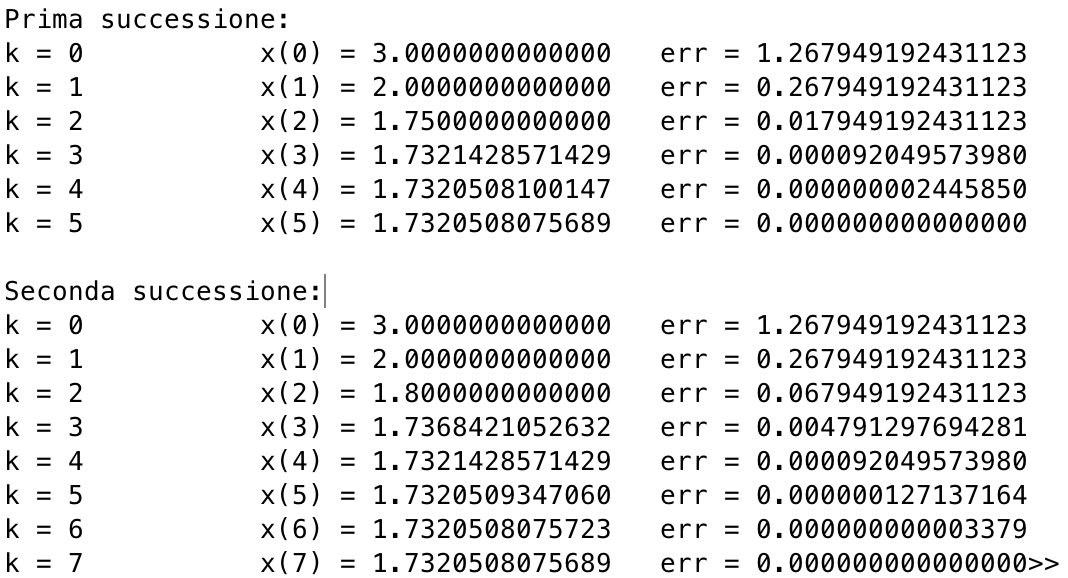
\includegraphics[width=12cm]{Capitolo1/es1_6.png}

	\end{flushleft}
